%====================================================================
%====================================================================
\subsection{From EM to variational EM to Monte-Carlo EM} 
\frame{\frametitle{Joint species distribution model} 

  \paragraph{Data.} $n$ sites, $p$ species, 
  \begin{itemize}
    \item $x_i =$ vector of covariates for site $i$
    \item $Y_i = (Y_{i1}, \dots Y_{ip}) =$ abundance vector in site $i$
  \end{itemize}

  \bigskip \pause
  \paragraph{Poisson log-normal (PLN) model.} 
  \begin{itemize}
    \setlength{\itemsep}{.75\baselineskip}
    \item Latent layer: 
    $$
    (Z_i)_{1 \leq i \leq n} \text{ iid } \sim \Ncal_p(0, \Sigma)
    $$
    \item Observed layer: counts $(Y_{ij})_{1 \leq i \leq n, 1 \leq j \leq p} \text{ indep} \mid Z$
    $$
    Y_{ij} \mid Z \sim \Pcal\left(\exp(o_{ij} + x_i^\top \beta_j + Z_{ij})\right)
    $$
    $o_{ij} =$ given 'offset' term, accounting for the samplign effort
    \item Parameters $\theta = (\beta, \Sigma)$:
    $$
    \beta_j = \text{abiotic interactions}, \qquad 
    \Sigma = \text{biotic interactions}
    $$
  \end{itemize}

}

%====================================================================
\frame{\frametitle{An example}

  \paragraph{A typical dataset.} 
  \begin{itemize}
    \setlength{\itemsep}{.75\baselineskip}
    \item Fish species from the Barents sea \refer{FNA06}.
    \item $n = 89$ sites, $p = 30$ species, $d = 4$ covariates (latitude, longitude, temperature, depth)
  \end{itemize}
  
  \bigskip \bigskip \pause
  \paragraph{Deciphiring between abiotic and biotic effects.} 
  $$
  \begin{tabular}{ccc}
    Covariate effects & 
    Correlation induced & 
    Between species \\
    $\widehat{B}$ & 
    by the environment & 
    correlation  $\widehat{\Sigma}$ \\
    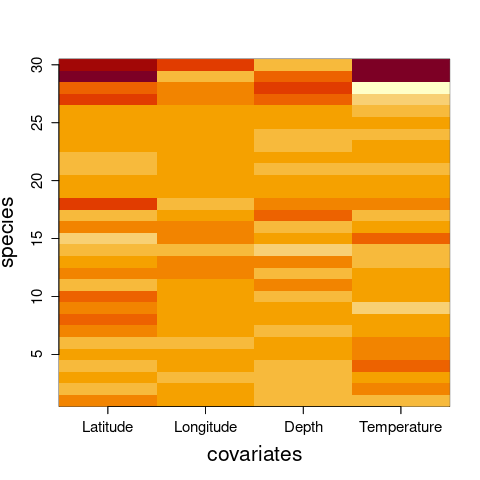
\includegraphics[width=.25\textwidth, trim=0 10 20 10, clip=]{\figbayes/FigUVSQ-BarentsFish-coeffAll-woIntercept-specOrderTRUE} & 
    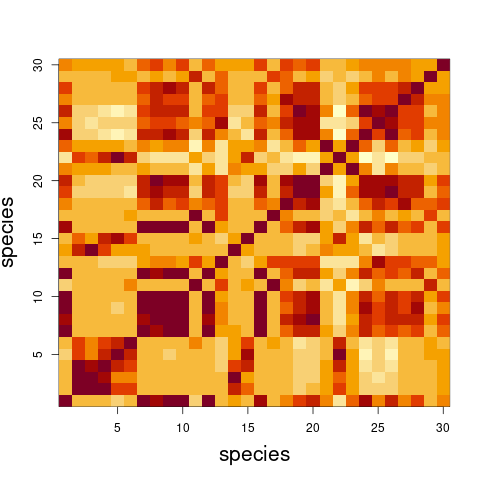
\includegraphics[width=.25\textwidth, trim=0 10 20 10, clip=]{\figbayes/FigUVSQ-BarentsFish-corrPred-specOrderTRUE} & 
    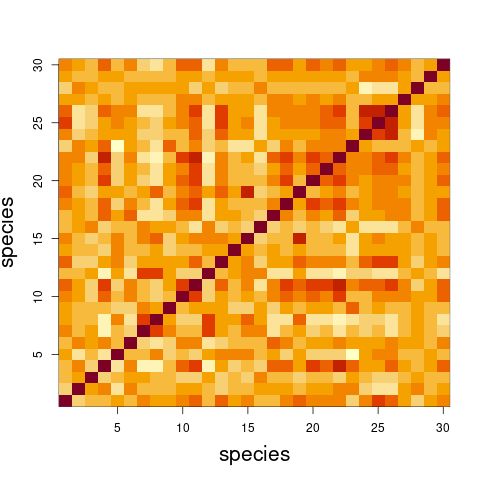
\includegraphics[width=.25\textwidth, trim=0 10 20 10, clip=]{\figbayes/FigUVSQ-BarentsFish-corrAll-specOrderTRUE}
  \end{tabular}
  $$

}

%====================================================================
\frame{\frametitle{Inference} 

  \paragraph{Maximum likelihood inference via EM.} \refer{DLR77}
  $$
  \theta^{(h+1)} 
  = \underset{\text{\normalsize \emphase{M step}}}{\underbrace{\argmax_\theta}} \; \underset{\text{\normalsize \emphase{E step}}}{\underbrace{\Esp_{\theta^{(h)}}}}[\log p_\theta(Y, Z) \mid Y]
  $$
  \begin{itemize}
    \setlength{\itemsep}{.75\baselineskip}
    \item The E step requires some knowledge about $p_\theta(Z \mid Y)$
    \item Which turns out to be intractable for the PLN model.
  \end{itemize}
  
  \bigskip \pause
  \paragraph{Variational EM \refer{WaJ08,BKM17}.} % Replace the E step with an approximation step, i.e.
  \begin{itemize}
    \setlength{\itemsep}{.75\baselineskip}
    \item \pause Choose a class $\Qcal$ of approximate (parametric) distributions and a divergence measure $D[q \| p]$ (e.g. $KL[q \| p]$)
    \item \pause \emphase{VE} step (approximation):
    $
    q^{(h+1)} = \argmin_{q \in \emphase{\Qcal}} \emphase{D}\left[q(Z) \| p_{\theta^{(h)}}(Z \mid Y)\right]
    $
    \item \pause \emphase{M} step (update):
    $
    \theta^{(h+1)} = \argmax_\theta \Esp_{\emphase{q^{(h+1)}}}\left[\log p_\theta(Y, Z)\right]
    $
    \\ ~
    \item \pause If $D = KL$, a lower bound of $\log p_\theta(Y)$ ('ELBO') increases at each step 
  \end{itemize}

}

%====================================================================
\frame{\frametitle{VEM for the Poisson log-normal model}

  \paragraph{Approximation class.} Gaussian approximation \refer{CMR18a,CMR19}
  $$
  q(Z) = \prod_{i=1}^n \Ncal(Z_i; m_i, S_i)
  $$
  \begin{itemize}
  \item Parameter estimate $\widehat{\theta} = (\widehat{\Sigma}, \widehat{\beta})$, 
  \item Approximate conditional distribution $Z_i \mid Y_i \approx \Ncal(\widetilde{m}_i, \widetilde{S}_i)$, 
  \item Lower bound $ELBO(\widehat{\theta}, \widetilde{m}, \widetilde{S})$ (R package \url{PLNmodels})
  \end{itemize}
  
  \bigskip \pause
  \paragraph{Properties.}
  \begin{itemize}
    \setlength{\itemsep}{.75\baselineskip}
    \item Reasonably easy to implement, fast, empirically accurate
    \item But very few theoretical guaranties, does not enjoy the general properties of maximum likelihood (consistency, asymptotic normality, etc.) \\
    \medskip 
    $\to$ No measure of uncertainty (\emphase{no test, no confidence interval}) 
    \item Can we build upon variational inference to achieve 'genuine' statistical inference?
  \end{itemize}
  
}

%====================================================================
\frame{\frametitle{Toward genuine maximum likelihood inference \refer{StR24}}

  \paragraph{Monte Carlo EM (MCEM).} \refer{CeD85} When $p(Z \mid Y)$ can be sampled from:
  \begin{itemize}
    \item \emphase{MCE} step: Sample $(Z^m)_{m = 1 \dots M} \overset{iid}{\sim} p_{\theta^{(h)}}(Z \mid Y)$, then estimate
    $$
    \widehat{Q}(\theta \mid \theta^{(h)}) := \frac1{M} \sum_{m=1}^M \log p_\theta(Y, Z^m)
    $$
    \item \emphase{M} step: Update
    $$
    \theta^{(h+1)} = \argmax_\theta \widehat{Q}(\theta \mid \theta^{(h)}) 
    $$
  \end{itemize}

  \bigskip \bigskip \pause
  \paragraph{Importance sampling. }
  When $p(Z \mid Y)$ can not be sampled from:
  \begin{itemize}
   \item Sample $(Z^m)_{m = 1 \dots M} \overset{iid}{\sim} q^{(h)}(Z)$, $q^{(h)} =$ proposal,
   \item Compute the non-normalized weights $\rho_m^{(h)} = p_{\theta^{(h)}}(Y, Z^m) \left/ q^{(h)}(Z^m)\right.$,
   \item \pause Estimate
    $$
    \widehat{Q}(\theta \mid \theta^{(h)}) := \sum_{m=1}^M \rho_m^{(h)} \log p_\theta(Y, Z^m) \; \left/ \; \sum_{m=1}^M \rho_m^{(h)} \right.,
    $$
  \end{itemize}

}

%====================================================================
\frame{\frametitle{Composite likelihood}

  \bigskip
  \paragraph{Importance sampling has a poor efficiency\footnote{Measured in terms of ESS $\simeq$ variance of the weights}} in 'large' dimension (say $p \geq 10, 15$) \\
  \medskip 
  $\to$ Need to reduce the sampling dimension

  \bigskip \bigskip \pause
  \paragraph{Composite likelihood.} 
  \begin{itemize}
    \item Build $B$ overlapping blocks $\Ccal_1, \dots \Ccal_B$, each containing $k$ species, 
    \item Define the composite log-likelihood as
    $$
    \cl_\theta(Y) = \sum_{b=1}^B \log p_\theta(Y^b), 
    \qquad
    \text{where} \quad 
    Y^b = [Y_{ij}]_{i = 1, \dots n, j \in \Ccal_b},
    $$
    \item \pause Then, the maximum composite likelihood estimator \refer{VRF11}
    $$
    \widehat{\theta}_{CL} = \argmax_\theta \cl_\theta(Y) 
    $$
    is consistent, asymptotically Gaussian with asymptotic variance given by
    \begin{align*}
      J(\theta) & = \Var_\theta[\nabla_\theta \cl_\theta(Y)], 
      \qquad \qquad 
      H(\theta) = - \Esp_\theta[\nabla^2_\theta \cl_\theta(Y)], \\
      \Var_\infty(\widehat{\theta}_{CL}) & = H^{-1}(\theta) J(\theta) H^{-1}(\theta).
    \end{align*} 
  \end{itemize}

}

%====================================================================
\frame{\frametitle{Proposed composite likelihood algorithm}

  \bigskip
  \paragraph{Proposition: EM applies for composite likelihood \refer{StR24}.}
  \begin{itemize}
    \item Because the latent variables $Z$ can be split in the same way as the observed abundances $Y$:
    $$
    Z^b = [Z_{ij}]_{i = 1, \dots n, j \in \Ccal_b},
    $$
    \item The EM decomposition applies within each block.
  \end{itemize}

  \bigskip \bigskip \pause
  \paragraph{Proposal for importance sampling.}
  \begin{itemize}
    \item Start with $q_b^{(1)}(Z^b) = \qt_{VEM}(Z^b)$
    \item Then update $q_b^{(h+1)}(Z^b)$ with the estimated mean and variance of $p_{\theta^{(h)}}(Z^b \mid Y^b)$.
  \end{itemize}

  \bigskip \bigskip \pause
  \paragraph{Building the blocks.} To guaranty the same precision for all estimates, one would ideally want that
  \begin{itemize}
    \item[$\beta_j$:] Each species $j$ belongs to the same number of blocks $\Ccal_1, \dots \Ccal_B$
    \item[$\sigma_{jj'}$:] Each pair of species $(j, j')$ appears in the same number of blocks 
    \item Same problem as the construction of a incomplete balanced block design\footnote{Not always possible: need to have $p \mid Bk$ and $p(p-1) \mid Bk(k-1)$} \goto{back:blocksCL} \label{sec:blocksCL}
  \end{itemize}

}

%====================================================================
%====================================================================
\subsection{Fish species from the Barents sea}
\frame{\frametitle{Fish species from the Barents sea}}
%====================================================================

%====================================================================
\frame{\frametitle{Simulation study}

  \paragraph{Main aim.} Assess normality 
  \begin{itemize}
    \item Test statistic $(\widehat{\theta} -\theta^*) \left/ \sqrt{\widehat{\Var}_\infty(\widehat{\theta})} \right.$ for the regression coefficients
    \item Criterion = $p$-value of the Kolmogorov-Smirnov test for normality
  \end{itemize}
  
  \bigskip \bigskip \pause
  \paragraph{Results.} $100$ sites, $3$ covariates, $100$ simulations
  \newcommand{\lagSim}{50} \newcommand{\nISsim}{200} \newcommand{\nIterSim}{1000}
  \newcommand{\simulParms}{-nIter\nIterSim-lag\lagSim-nIS\nISsim}
  $$
  \begin{tabular}{cccc}
    7 species & 10 species & 20 species & 50 species \\
    \includegraphics[width=.2\textwidth, trim=10 10 25 25, clip=]{\figStR/PvalKS-score-n100-d3-p7-parm1\simulParms} & 
    \includegraphics[width=.2\textwidth, trim=10 10 25 25, clip=]{\figStR/PvalKS-score-n100-d3-p10-parm1\simulParms} & 
    \includegraphics[width=.2\textwidth, trim=10 10 25 25, clip=]{\figStR/PvalKS-score-n100-d3-p20-parm1\simulParms} &
    \includegraphics[width=.2\textwidth, trim=10 10 25 25, clip=]{\figStR/PvalKS-score-n100-d3-p50-parm1\simulParms}  
  \end{tabular}
  $$
  FL = full likelihood, CL$k$ = composite likelihood$(k = \textcolor{gray}{2}, 3, 5, 7)$, \\
  \medskip
  \textcolor{gray}{VEM = pseudo Fisher information matrix based on the ELBO},  \\
  JK = jackknife variance estimate of $\Var(\widehat{\theta}_{VEM})$

}

%====================================================================
\frame{\frametitle{Fish species in the Barents sea}

  \newcommand{\nIterEx}{10000} \newcommand{\lagEx}{50} \newcommand{\nISex}{200}
  \newcommand{\exampleParms}{-nIter\nIterEx-lag\lagEx-nIS\nISex}
  \newcommand{\nIterSel}{\nIterEx} \newcommand{\lagSel}{20} \newcommand{\nISsel}{\nISex}
  \newcommand{\selectParms}{-nIS\nISsel-nIter\nIterSel-lag\lagSel}
  
  \bigskip
  \paragraph{Comparison of the estimates.}
  $$
  \begin{tabular}{ccc}
    $\widehat{B}$ & $\widehat{\Sigma}$ & ESS (CL5) \\
    \includegraphics[width=.25\textwidth, trim=10 10 25 50, clip=]{\figStR/Barents\exampleParms-compBeta-cem5-all} & 
    \includegraphics[width=.25\textwidth, trim=10 10 25 50, clip=]{\figStR/Barents\exampleParms-compSigma-cem5-all} & 
    \includegraphics[width=.25\textwidth, trim=10 10 25 50, clip=]{\figStR/Barents\exampleParms-ESS-cem5}     
  \end{tabular}
  $$

  \pause
  \paragraph{Significance.} Test statistics $\widehat{\theta} \left/ \sqrt{\widehat{\Var}_\infty(\widehat{\theta})} \right.$
  $$
  \begin{tabular}{ccc}
    $\widehat{B}$ & $\widehat{\Sigma}$ & $\text{cor}(\widehat{\Sigma})$ \\
    \includegraphics[width=.25\textwidth, trim=10 10 25 25, clip=]{\figStR/Barents\exampleParms-betaSignif-cem5} & 
    \includegraphics[width=.25\textwidth, trim=10 10 25 25, clip=]{\figStR/Barents\exampleParms-sigmaSignif-cem5} &
    \includegraphics[width=.25\textwidth, trim=10 10 25 25, clip=]{\figStR/Barents\exampleParms-corSigmaSignif-cem5}
  \end{tabular}  
  $$
}

